	Mediante la herramienta de análisis de Fourier provista por \texttt{SPICE Orcad} se analizó la variación de la distorsión armónica \texttt{THD} producida en la salida, en función de la frecuencia y amplitud de la señal de entrada. Los resultados obtenidos se resumen en la tabla.

\begin{table}[H]
	\centering
	\begin{tabular}{ccccc}
		\toprule
\multirow{2}{*}{Frecuencia} & \multicolumn{3}{c}{$P_{L,RMS}$} \\ 
		\cmidrule{2-4}
			& 4W & 30W & 42,5W \\
		\midrule
		\SI{1}{\kHz} & \num{0,005} & \num{0,016} & \num{0,018} \\
		\SI{20}{\kHz} & \num{0.053} & \num{0,066} & \num{0,099} \\
		\bottomrule
	\end{tabular}
	\caption{Valores de $\mathrm{THD}_{\%}$ para distintos valores de frecuencia y potencias sobre la carga.}
\end{table}


\begin{figure}[H]
	\centering
	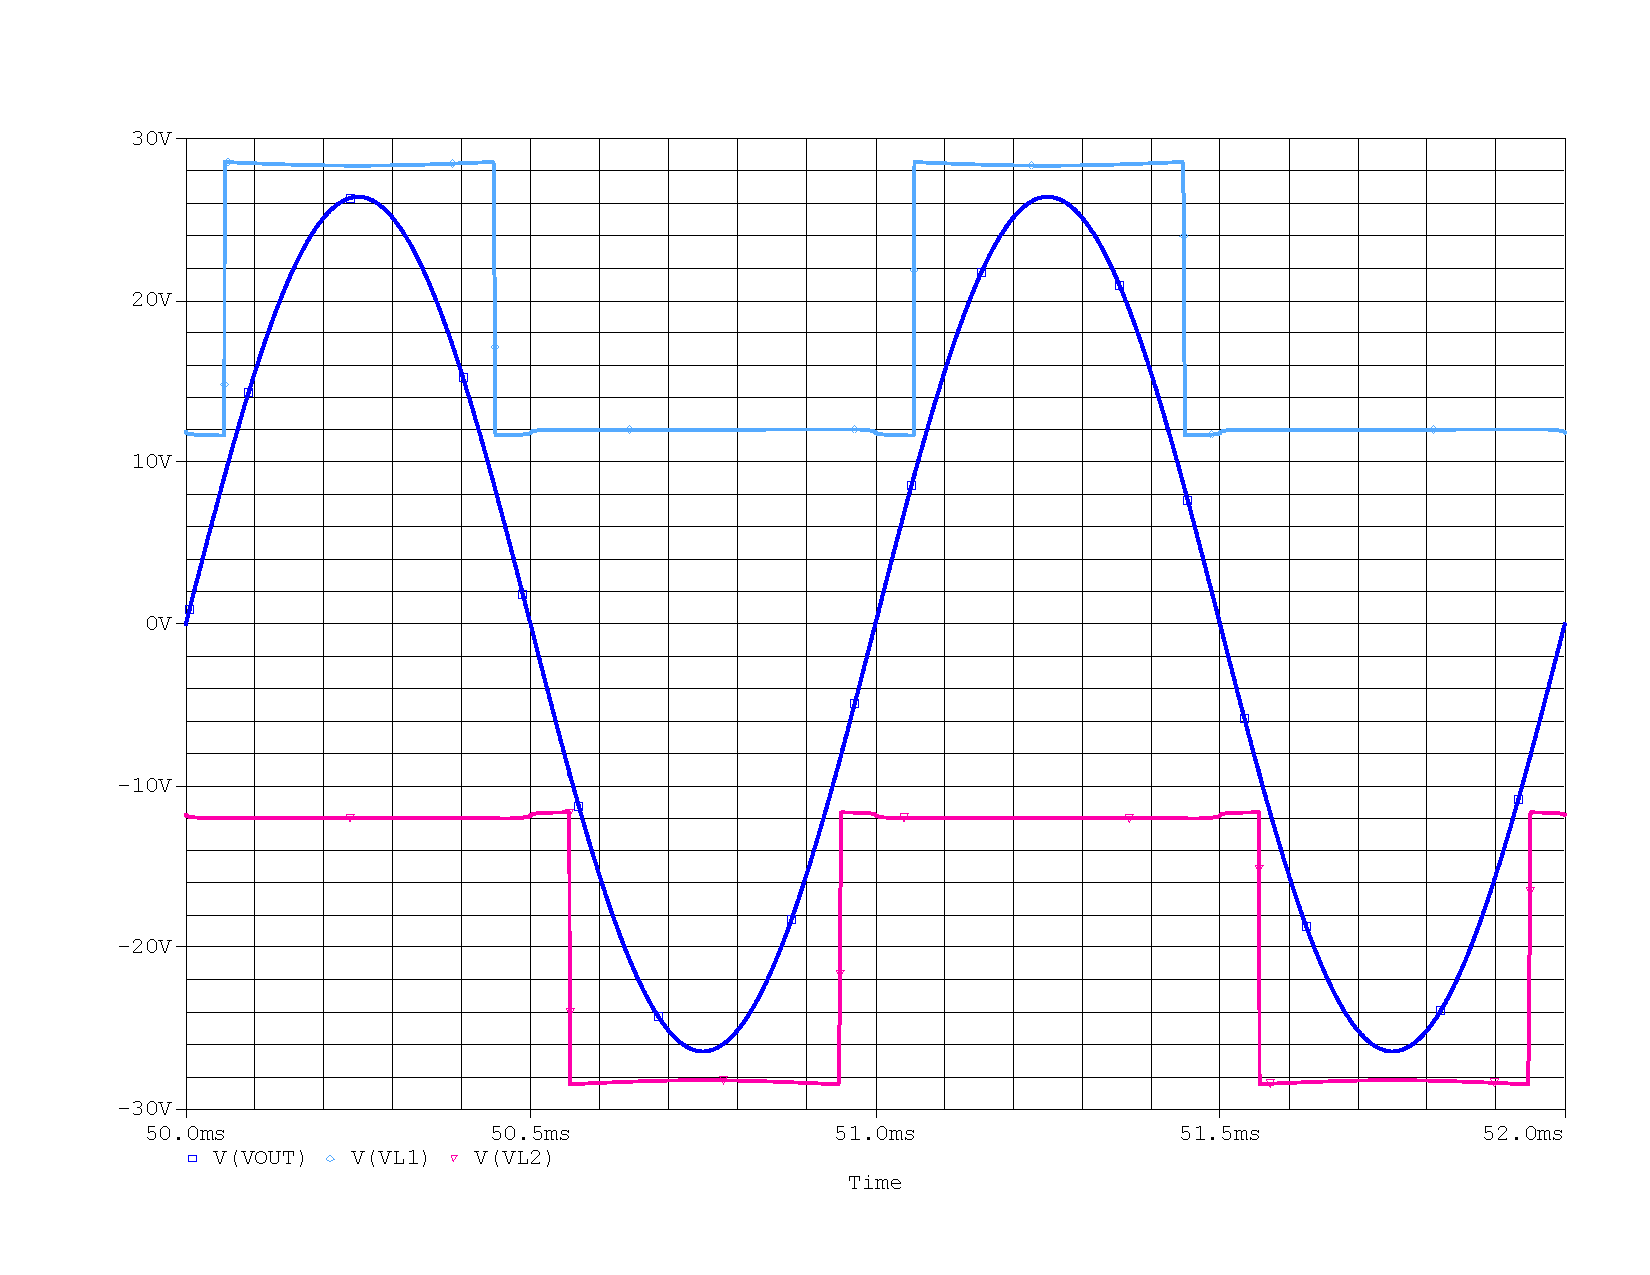
\includegraphics[scale=0.4]{sim_salida1k_max.pdf}
	\caption{Máxima excursión de salida sin recorte a \SI{1}{\kilo\hertz} $THD = \num{0.018}\%$.}
	\label{fig:sim_salida_1k_max}
	\end{figure}

\begin{figure}[H]
	\centering
	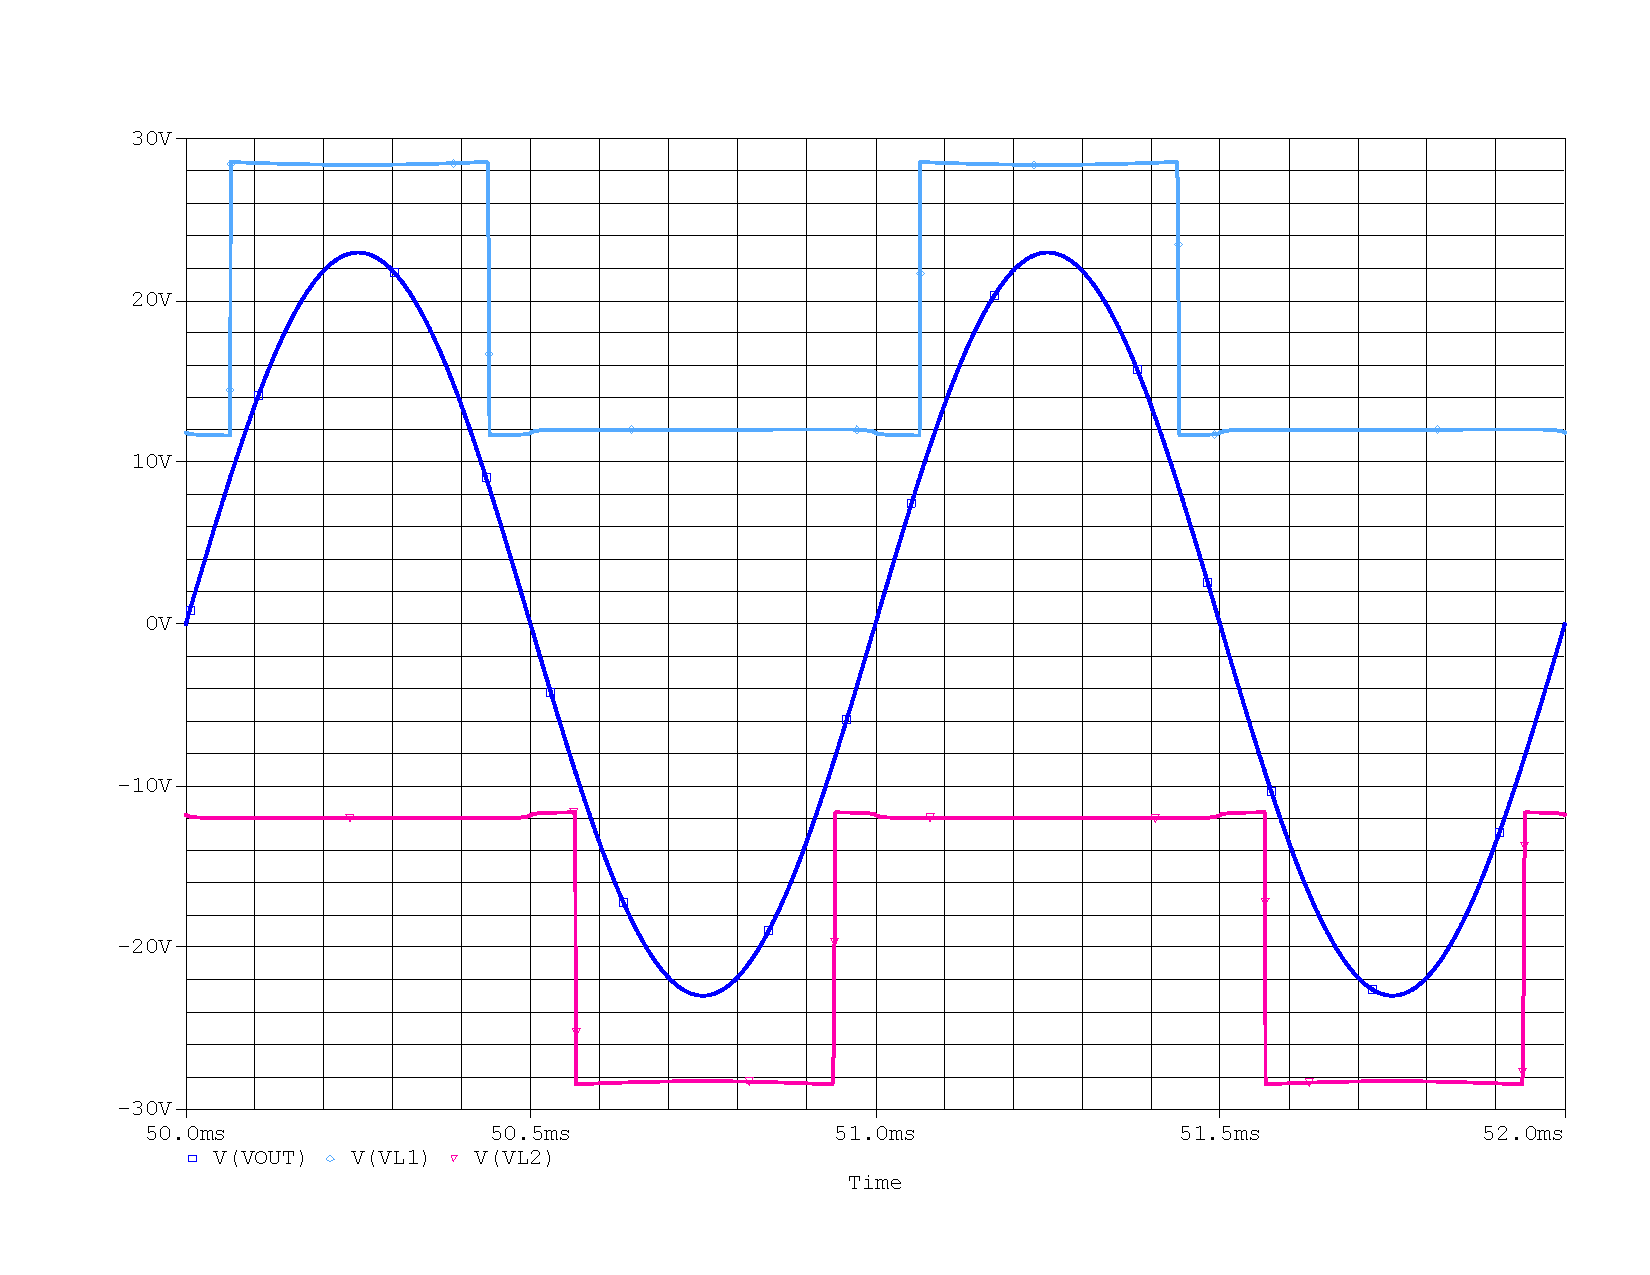
\includegraphics[scale=0.4]{sim_salida_1k_22V.pdf}
	\caption{22V, 1V, $THD=\num{0.016}\%$.}
	\end{figure}

\begin{figure}[H]
	\centering
	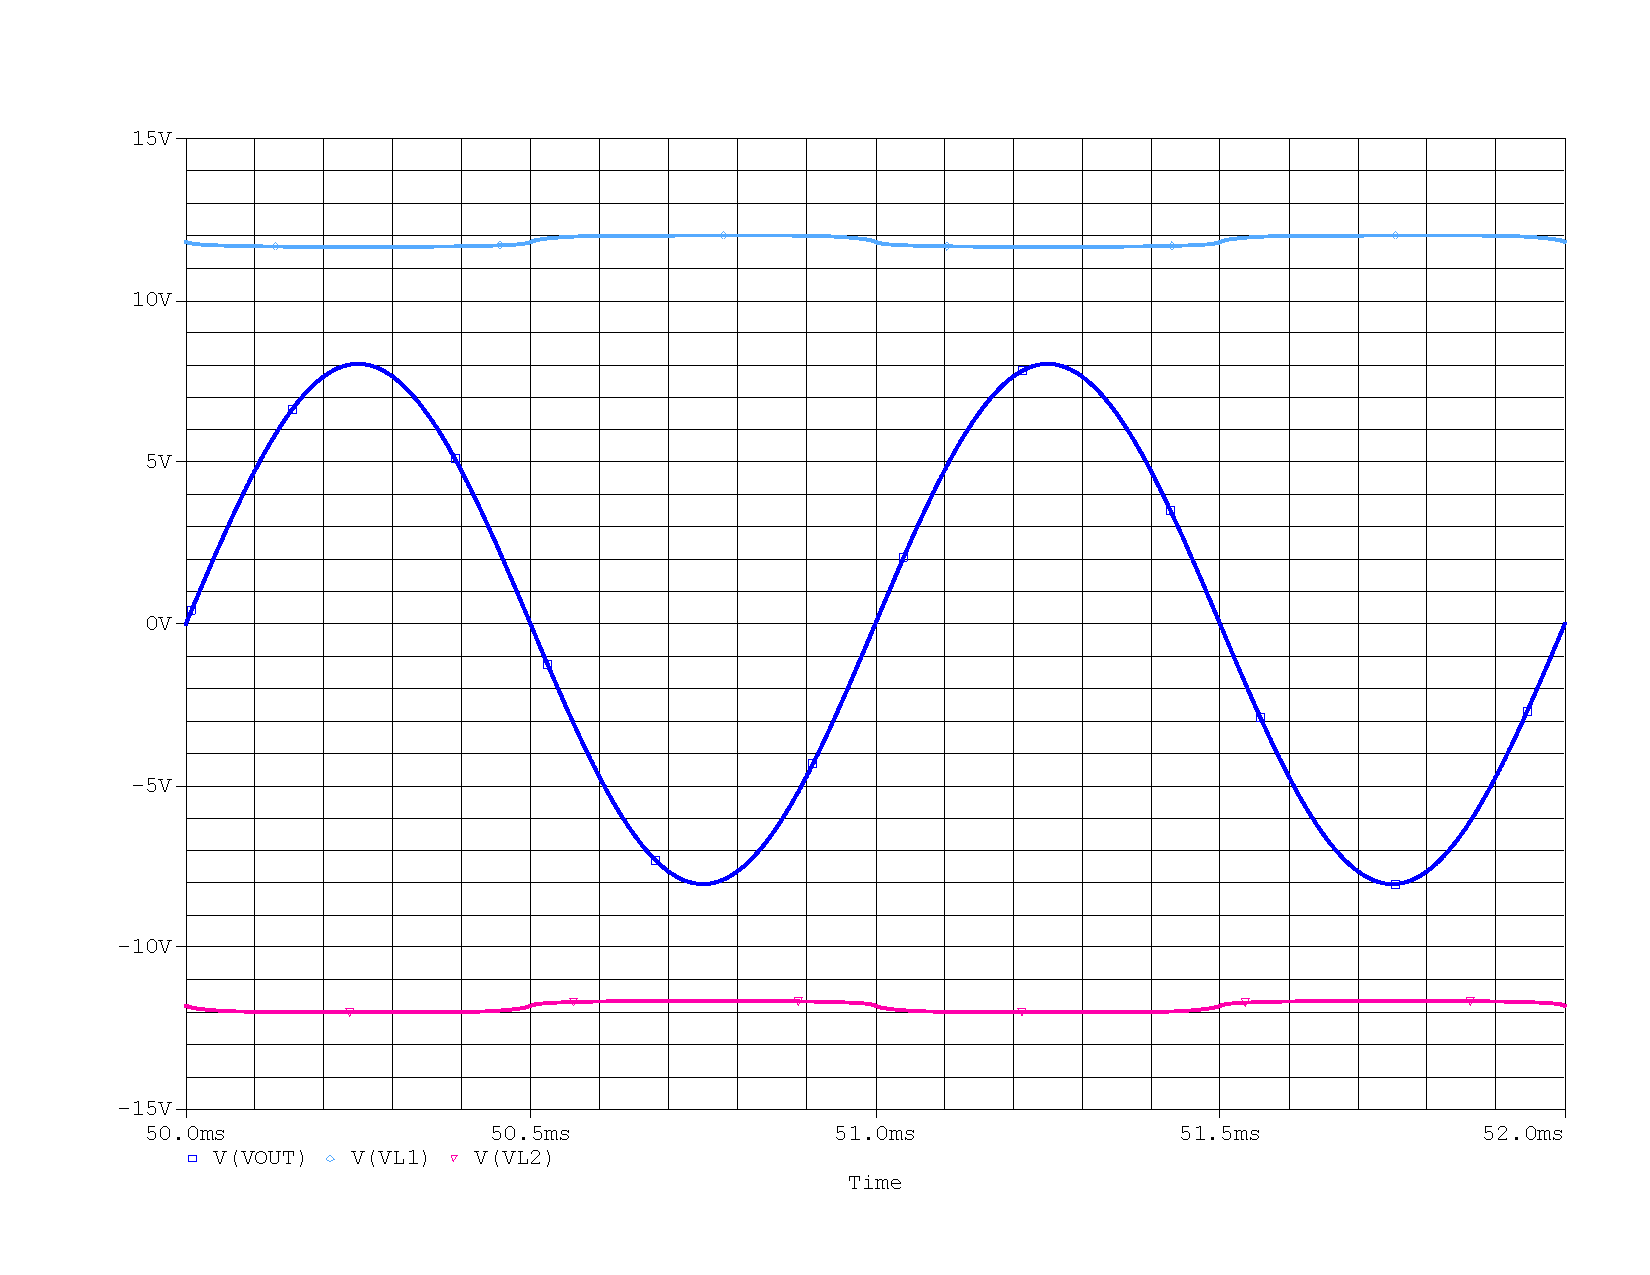
\includegraphics[scale=0.4]{sim_salida_1k_8V.pdf}
	\caption{8V, $\SI{.35}{\V}$, $THD=\num{0.005}\%$.}
\end{figure}

%%%% 20kHz
\begin{figure}[H]
	\centering
	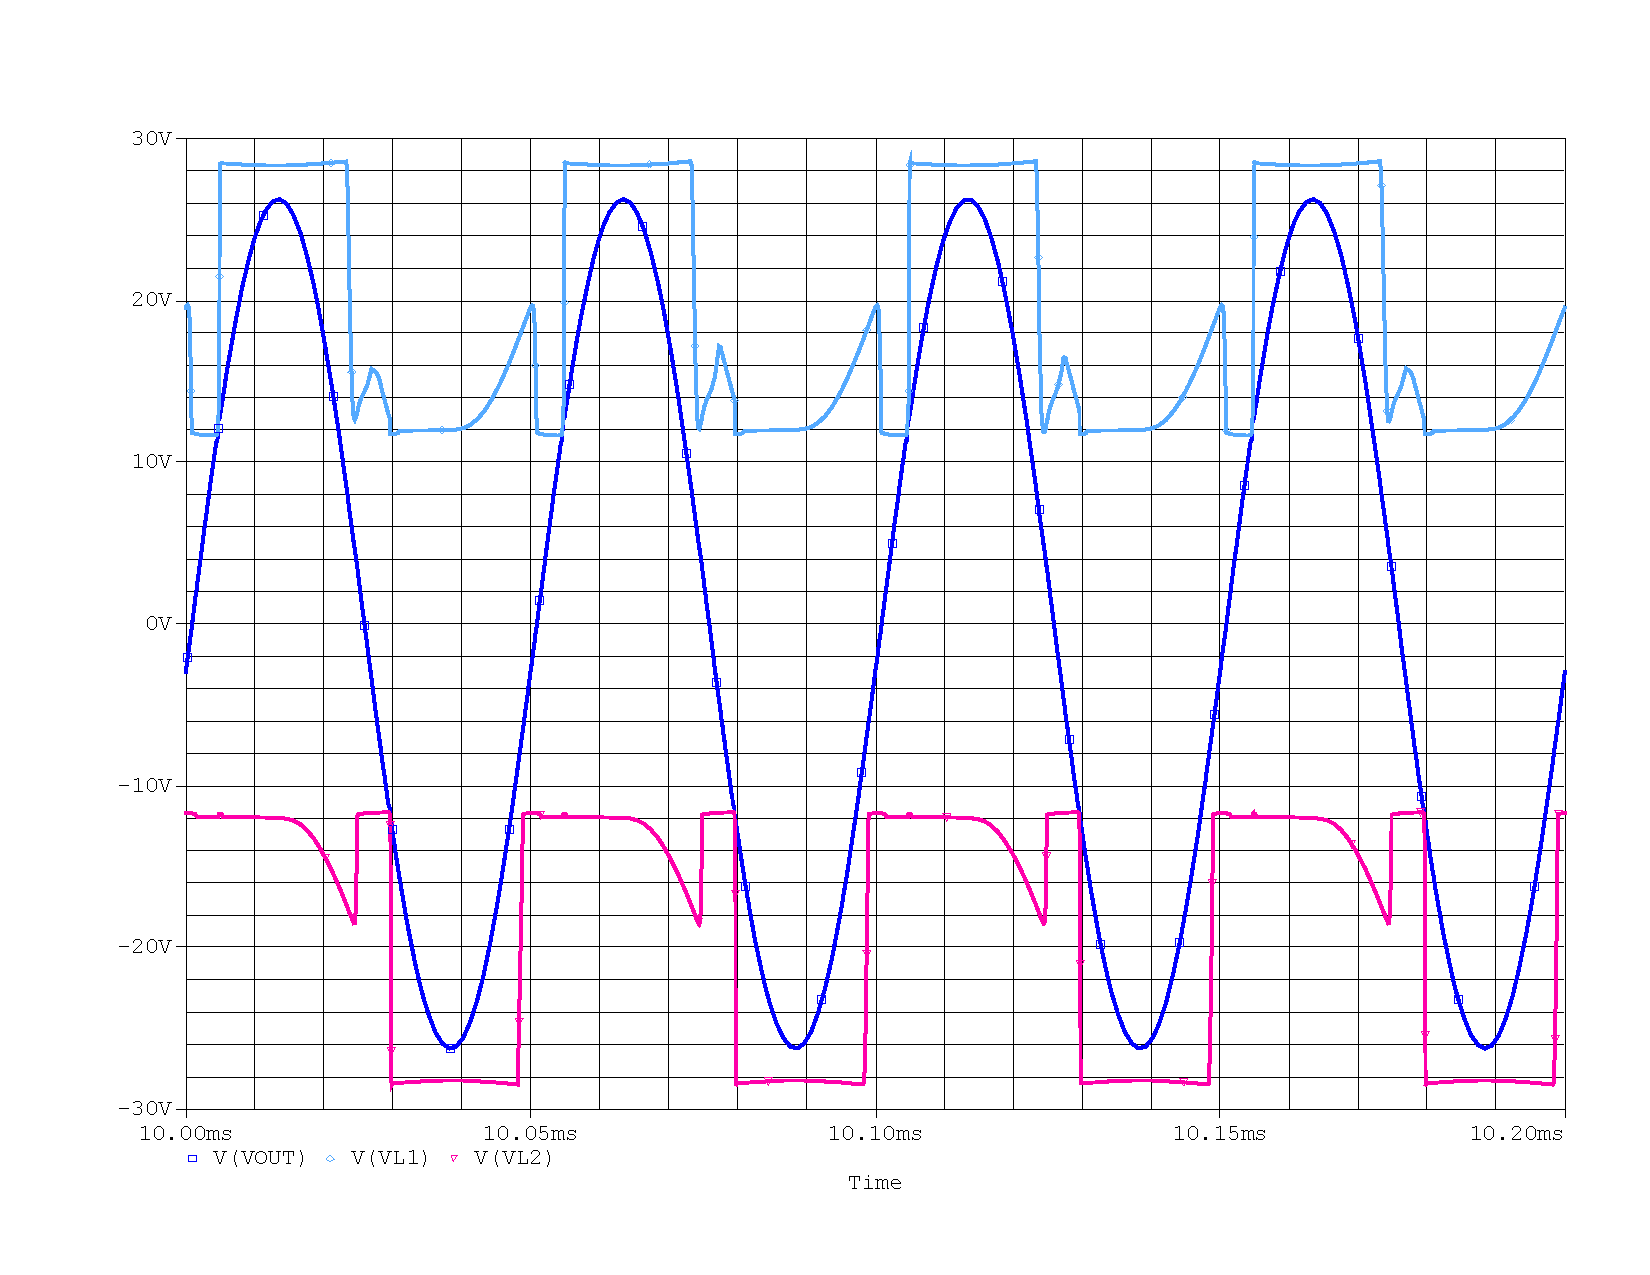
\includegraphics[scale=0.4]{sim_salida_20k_max.pdf}
	\caption{\SI{26.1}{\V}, \SI{0.35}{\V}, $THD=\num{0.053}\%$.}
\end{figure}

\begin{figure}[H]
	\centering
	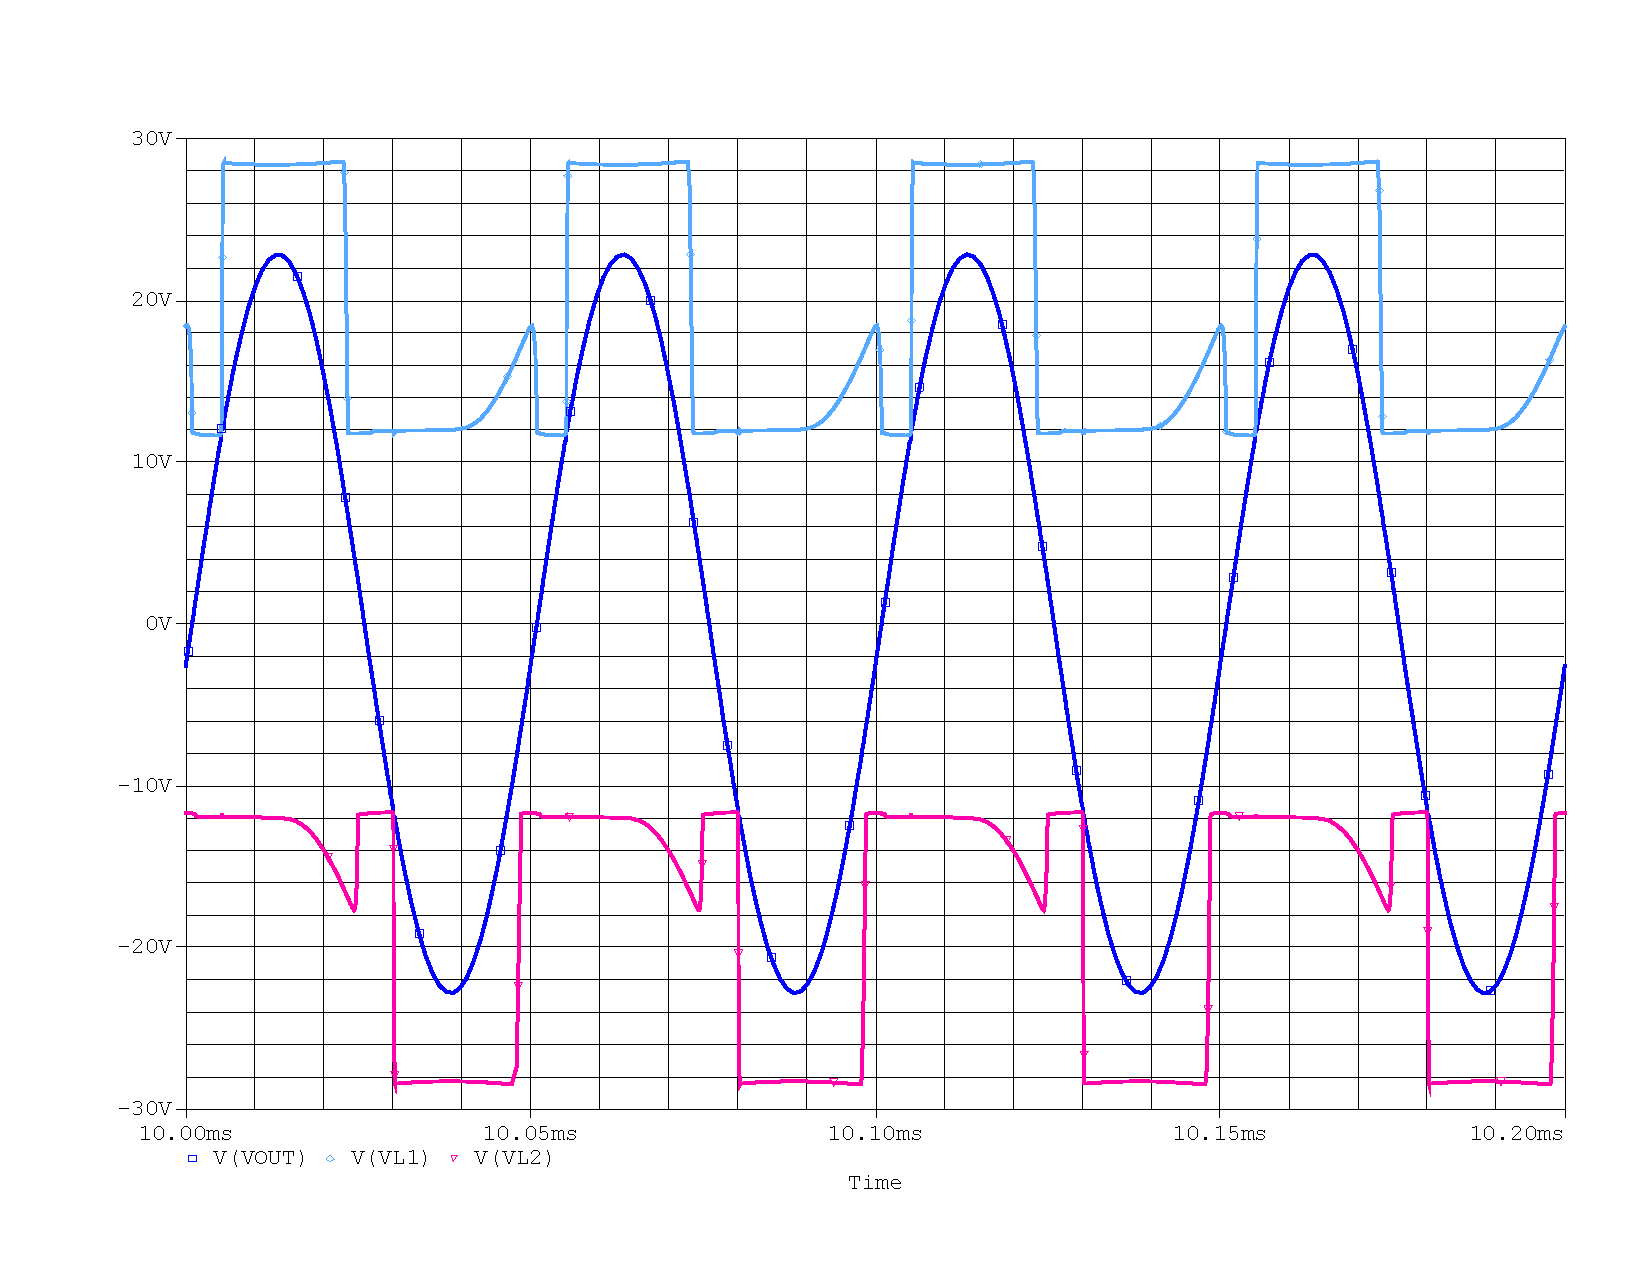
\includegraphics[scale=0.4]{sim_salida_20k_22V.pdf}
	\caption{\SI{22}{\V}, \SI{1}{\V}, $THD=\num{0.066}\%$.}
\end{figure}

\begin{figure}[H]
	\centering
	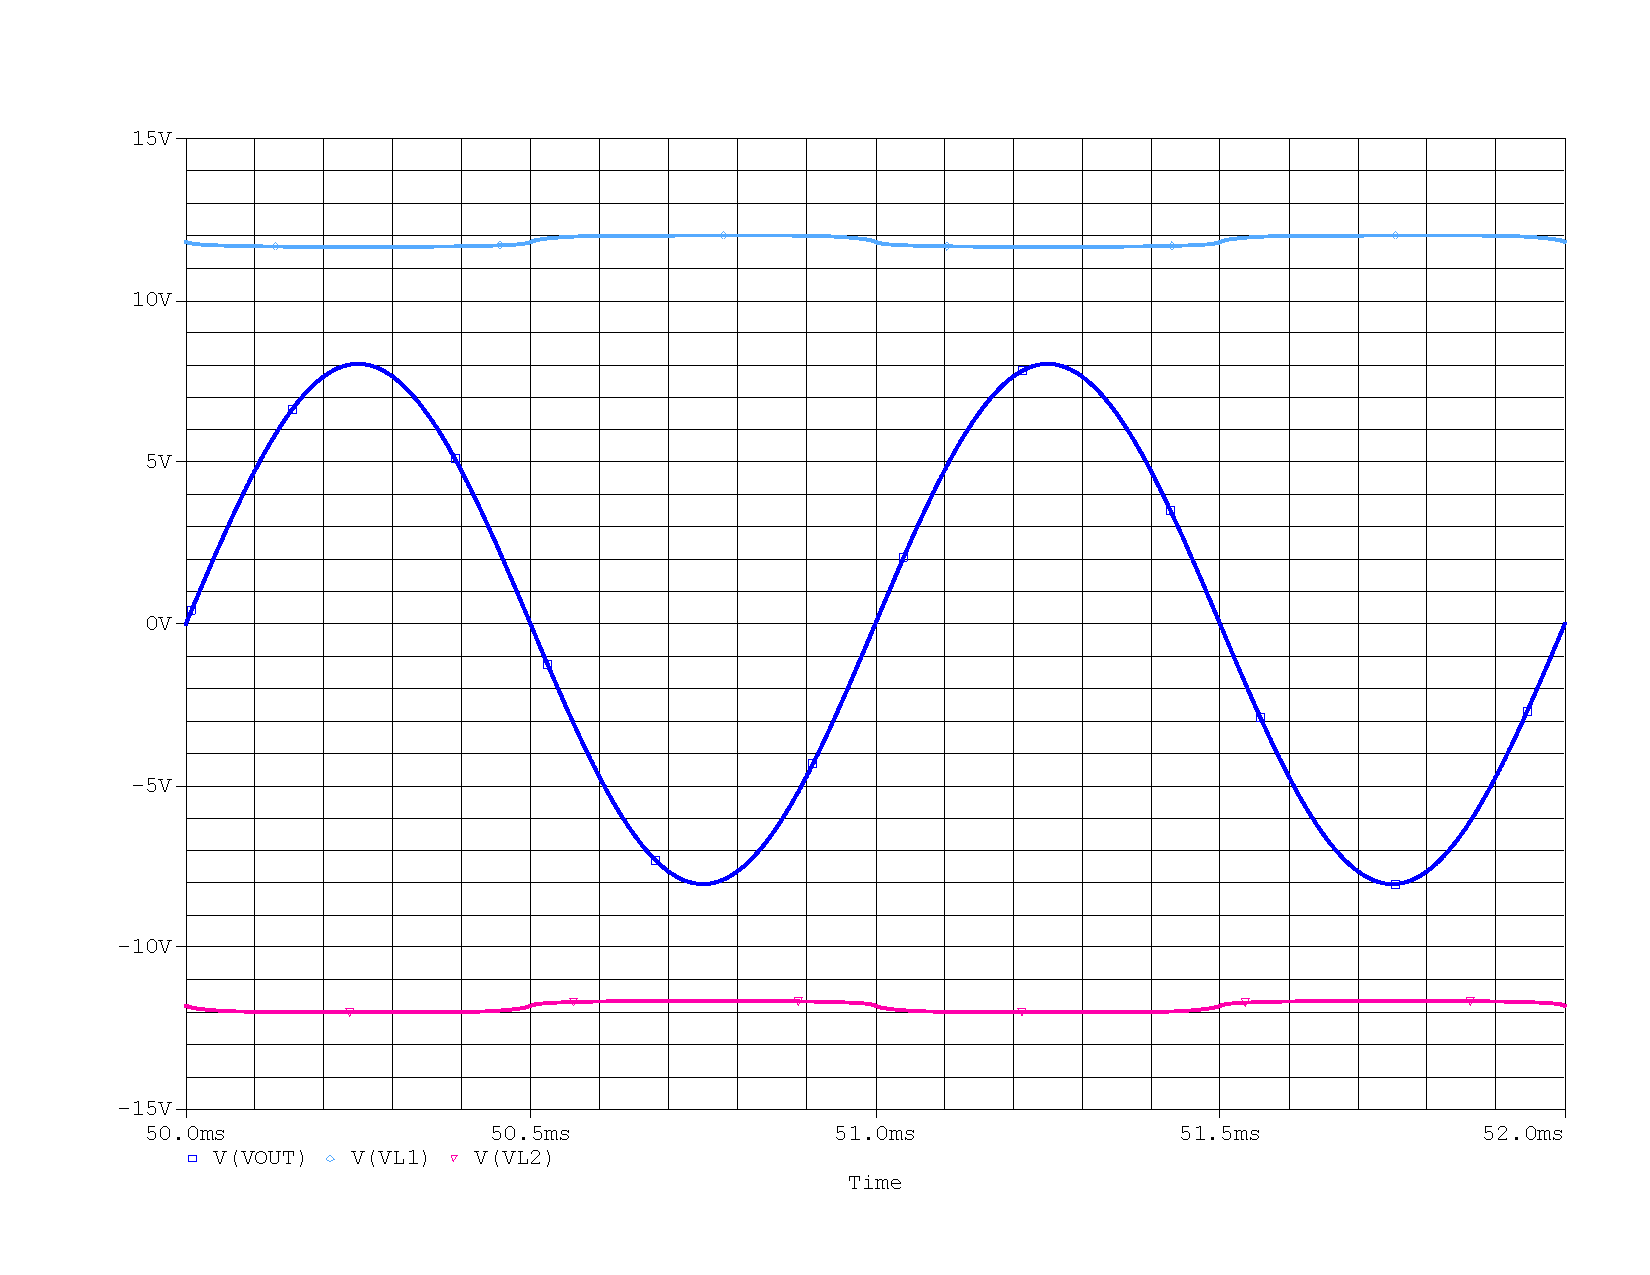
\includegraphics[scale=0.4]{sim_salida_1k_8V.pdf}
	\caption{\SI{8}{\V}, \SI{0.35}{\V}, $THD=\num{0.099}\%$.}
\end{figure}




